\section{\texorpdfstring{First time in
\emph{M16}}{First time in M16}}

\margininbox{M16}{
     \begin{itemize}
    \item Erik Bončina
    \item James "Tetley" Hooper
    \item Iztok Možir
    \end{itemize}}{\explo}

It was my first year on Mig and I was very excited to go caving and join
the ICCC on top. Till now, we were only caving in \passage{Primadona} while
staying at \passage{Kal}. One day Erik and I decided to go and rather than sleep
at \passage{Kal}, sleep on top with the English. We stayed up for a couple of
days. Our first caving trip was in \passage{M16}. Tetley took us to the
bottom of \passage{Sajeta}. From \passage{XXX} onwards Tetley was unsure of the rope and
said that his brains are telling him not to go further, but his heart
wants to go. Tetley descended \passage{Sajeta} first, followed by myself and then
Erik. When I arrived at the bottom, Tetley was acting really seriously
and said to me ``What are you doing here?'' I was bit confused why is he
asking me that and thought we should not follow him down. He then asked
me the same question couple of times which made me even more confused.
On the end I finally said to him, that I am here to cave. He then
replied ``If you are on holidays, \bignote{why are you here and not chasing girls
on Croatia beach?}'' We start laughing. Same happened to Erik.

On the way out Tetley was rushing us to get out (we were leading the way
to memorise the cave), as he did not want to miss the call out. At that
time we did not know what a call out was and so we speeded up. On the
end I was really tired, but it was worth it.

\name{Izi Možir}

\begin{pagefigure}
\checkoddpage \ifoddpage \forcerectofloat \else \forceversofloat \fi
   \centering
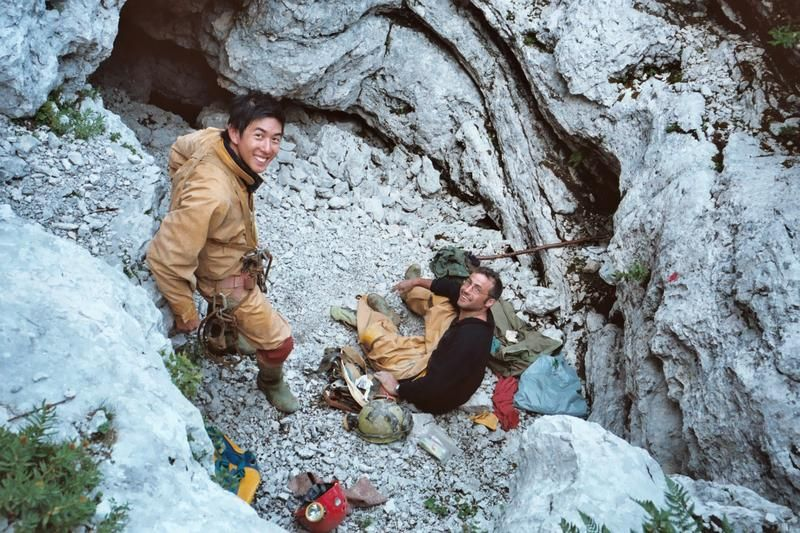
\includegraphics[width = 0.9\textwidth]{2007/m16/jarvist frost gr1 film1 -004_1--orig.jpg}
\caption{Alvin and Tetley in the entrance shakehole to \protect\passage{M16}. \pic{Jarvist Frost}}
\end{pagefigure}
